\documentclass{article}
\usepackage[utf8]{inputenc}
\usepackage{setspace}
\usepackage{graphicx} % Required for images
\usepackage{xcolor}   % Required for text coloring
\usepackage{amsmath}  % For advanced math formatting (if needed)

% Title, author, and date
\title{\textbf{Paragraph Writing For Class 10}}
\author{\textbf{Dr. Khastagir Government Girls' High School}}
\date{}

\begin{document}

% Title page
\maketitle

% Centered image
\begin{center}
    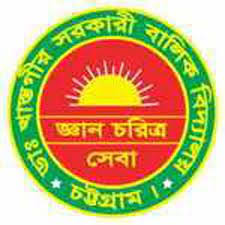
\includegraphics[width=0.2\textwidth]{images.jpg} % Ensure the image file exists in the same directory or specify the correct path
\end{center}

% Attribution line
\subsection*{\begin{center}\normalfont This document was made by Sakib\end{center}}

\subsection*{\begin{center}\LARGE A Book Fair\end{center}}

A book fair is a fair where different types of books are brought for sale or display. Nowadays, book fairs have become very popular. A book fair is usually held in the months of January and February. In our country, it is held in almost all cities and towns. The largest book fair is organized by Bangla Academy on the occasion of 21st February. It has created a sense of interest in books amongst the general masses. 

In a book fair, hundreds of pavilions are set up. All sorts of books—fiction, textbooks, dramas, children's books, reference books, etc.—are displayed. There are also food and drink stalls. A book fair becomes crowded, especially in the evening. Both male and female customers gather at a book fair. Writers also visit the fair regularly. Seminars and cultural programs are also held. 

The main purpose of a book fair is not just sales but to offer a rare opportunity to assess the advancement made in the publication of books. It helps to create new writers as well as new readers. It inspires people to form the habit of reading. A book fair bears testimony to the refined tastes and national culture of a country. A book fair reminds us that books are our best companions. They change our outlook on life and widen our domain of knowledge. It is books that help us forget jealousy, malice, and superstition. We get these best friends at a cheaper rate from a book fair. Thus, a book fair is of great value and helps to build an enlightened nation.

A book fair is a fair where different types of books are brought for sale or display. Nowadays, book fairs have become very popular. A book fair is usually held in the months of January and February. In our country, it is held in almost all cities and towns. The largest book fair is organized by Bangla Academy on the occasion of 21st February. It has created a sense of interest in books amongst the general masses. 

In a book fair, hundreds of pavilions are set up. All sorts of books—fiction, textbooks, dramas, children's books, reference books, etc.—are displayed. There are also food and drink stalls. A book fair becomes crowded, especially in the evening. Both male and female customers gather at a book fair. Writers also visit the fair regularly. Seminars and cultural programs are also held. 

The main purpose of a book fair is not just sales but to offer a rare opportunity to assess the advancement made in the publication of books. It helps to create new writers as well as new readers. It inspires people to form the habit of reading. A book fair bears testimony to the refined tastes and national culture of a country. A book fair reminds us that books are our best companions. They change our outlook on life and widen our domain of knowledge. It is books that help us forget jealousy, malice, and superstition. We get these best friends at a cheaper rate from a book fair. Thus, a book fair is of great value and helps to build an enlightened nation.

\subsection*{\begin{center}\LARGE A Moonlit Night\end{center}}

A moonlit night, when the full moon shines in its entire glory in the sky, is really charming and enjoyable. It is truly a night of dreams and presents a beautiful sight. In autumn, the sky remains cloudless, and the moon looks like a big silver disc in the sky. The shiny light of the moon floods the earth and the sky. The moon's rays, reflecting on seas, rivers, ponds, and hills, create a magical spell. When the moon pours her light on the waves of water, it sparkles like diamonds. The smooth rays of the moon bring peace to our eyes and minds.

On a moonlit night, the grand sights of canals, rivers, and tanks cannot be described in words. The whole of nature looks bright and appears bathed in celestial light. The natural beauty of a moonlit night can be better realized than described. People of all ages enjoy a moonlit night. Young boys play, little kids have fun and amuse themselves, and some people visit their neighbors' houses during this time. It seems as though the whole of nature has taken on a new form, and everywhere is bright, bright, and bright.

A moonlit night spreads a feeling of joy throughout all objects of nature. It is especially enjoyable for newly married couples. Poets of all languages have sung highly of a moonlit night. Even enemies forget their enmity, forming groups to converse on various subjects. A moonlit night reminds us of the mystery of Allah's creation. We can appreciate the moonlit night as offering a charming sight to all living beings. Indeed, a moonlit night is pleasant and fine.
\newpage
\subsection*{\begin{center}\LARGE A School Magazine\end{center}}

A school magazine is a magazine that contains the writings of the teachers and students of a school. Almost every well-established school publishes a magazine every year. It gives a view of the life of the school and reveals the creative genius of the students. It contains poems, articles, and short stories—all written by the teachers and students.

The publication of a school magazine is a very difficult task. The editor and his assistants have to work hard to publish the magazine. The magazine committee invites writings from students and teachers. The editorial board selects the qualified ones for printing. 

The school magazine serves many useful purposes. The most important is that it brings out the latent creative talents of the students and thus helps them to become great writers. A student feels proud and happy when he finds his own writing in print. The school magazine also reflects the academic and co-curricular activities of the school. It is a treasure island for the students. The students can learn many things from the school magazine. 

In a word, the school magazine mirrors the school.
\subsection*{\begin{center}\LARGE A Winter Morning\end{center}}

In Bangladesh, there are six different seasons. Winter is the coldest of them all. As a result, winter mornings are inherently remarkably cold. It's normally a foggy morning, with thick fog all around. On such a winter morning, the fog can be so dense that nothing can be seen even from a short distance. Even the sun's beams are unable to penetrate the fog. Everything is engulfed in deep fog and bitter cold. Nature appears gloomy, and everything appears hazy.

Due to the gloomy weather and harsh cold, people often wake up late, and children are frequently late for school. When heading to their place of employment and performing their jobs, people need to start their day early in the cold weather. People living in villages and facility-deprived people living on city streets are the ones who suffer most on such mornings due to a lack of warm clothing.

When the sun comes up and unveils the fog, people, particularly the elderly and children, seek comfort in the sun to cure their colds. Dewdrops that fall on grass, leaves, and flowers at midnight sparkle like pearls in the early sun. Date juice vendors can frequently be spotted selling date juice on the corners of streets. A sip of such a sweet drink is quite refreshing. Eating homemade cakes (Pitha) and date juice while relaxing in the warmth of the early morning sun is such a pleasant and lovely feeling that most people would love to have, which is why most children enjoy winter mornings so much.
\subsection*{\begin{center}\LARGE Climate Change\end{center}}

Climate change is a change in global or regional climate patterns. It refers to the rise in average surface temperatures on Earth. Climate change is the most discussed issue in the present world and attracts the attention of people from all walks of life at both local and global levels. Environmental scientists and activists are mostly concerned about the quick changes in climate.

The main cause of climate change is the burning of fossil fuels, such as oil and coal, which emits greenhouse gases into the atmosphere, mostly carbon dioxide. Other human activities, such as agriculture and deforestation, also contribute to the increase of greenhouse gases that cause climate change. The climate is changing rapidly, leaving bad impacts on developing countries. These impacts include temperature rise, greenhouse gas emissions, irregular rainfall, salinity intrusion, floods, cyclones, storm surges, and droughts, among others. Undoubtedly, these factors seriously affect the agriculture and livelihood of developing countries.

Bangladesh, due to its geographical location, is likely to be the most affected. A one-meter sea-level rise will submerge about one-third of the total area of Bangladesh, displacing 25–30 million people. To reduce the adverse impacts of climate change, people should become more aware. We should plant more trees and stop using harmful chemicals to mitigate the effects of climate change. Students should take responsibility to protect the environment and raise awareness.

In fact, to reduce the adverse impacts of climate change, all of us must work together; otherwise, our existence will be at stake.

\subsection*{\begin{center}\LARGE Artificial Intelligence (AI)\end{center}}

Artificial Intelligence (AI) is a type of technology that allows machines and computers to think and work like humans. It helps make our lives easier by doing tasks that are difficult or boring for us. For example, when you use your phone, the voice assistants like Google Assistant and Siri answer your questions. These assistants are powered by AI. 

AI also helps machines and robots perform tasks that humans do, such as driving cars, diagnosing diseases, or even writing stories. Nowadays, AI is used in many fields, including healthcare, education, and transportation. For instance, in hospitals, AI helps doctors identify illnesses faster, which saves time and lives. In cars, AI is used for self-driving, which means the car can drive itself without needing a human. AI is also used to recommend videos or products you might like, based on what you have already watched or purchased.

While AI is making life easier, some people are worried that it could take away jobs from humans. But, AI is here to stay, and it is helping people to do their work better and faster. Many people believe that AI will continue to grow and improve, making life easier for everyone. If we use it carefully, AI can help us solve many problems and improve our daily lives.
\subsection*{\begin{center}\LARGE Dengue Fever\end{center}}

Dengue fever, a mosquito-borne disease caused by a virus transmitted through Aedes mosquito bites, primarily \textit{Aedes aegypti}, poses a significant health threat in many regions. Symptoms typically appear 3 to 14 days post-infection, including high fever, intense headaches, vomiting, joint and muscle pain, and sometimes skin rashes. Most individuals recover within two to seven days with proper care, but the illness can progress to severe forms like dengue hemorrhagic fever, marked by bleeding, low platelet counts, and plasma leakage, or dengue shock syndrome, which causes dangerously low blood pressure. These complications can be life-threatening if not addressed promptly.

The virus has five distinct types, and infection with one grants lifelong immunity to that strain but only temporary protection against the others. Subsequent infections with different types heighten the risk of severe outcomes, making multiple exposures particularly dangerous. Diagnosis relies on tests detecting the virus or its RNA-resistant antibodies in the blood. Vaccines exist in some countries but are most effective for those previously infected, limiting their widespread use.

Prevention hinges on avoiding bites and controlling Aedes mosquito populations. These mosquitoes breed in stagnant water found in tree hollows, coconut shells, cups, and rooftops, so eliminating these sites is crucial. They bite mainly in the early morning and evening, when protective measures like mosquito nets—especially for children—and long clothing are recommended. For treatment, rest, hydration, and paracetamol for fever are standard, while severe cases may require intravenous saline or blood transfusions. NSAIDs and antibiotics should be avoided to prevent worsening symptoms.

In Bangladesh, dengue claims lives yearly, underscoring the need for awareness and action. Government efforts to curb the disease are notable, but collective responsibility—through education, sanitation, and prevention—can reduce infections and fatalities. Dengue demands vigilance; with the right steps, its impact can be minimized effectively.
\newpage
\subsection*{\begin{center}\LARGE Deforestation\end{center}}

Deforestation is the practice of removing trees and vegetation from forest regions. A variety of factors can be blamed for this, including population growth, lack of awareness, housing requirements, and industrial needs. Deforestation is a serious concern for our planet's future. 

As the population continues to increase, first, we need more habitation areas and cultivable land to accommodate this additional population. As a consequence, people cut down trees to build houses and clear forests for farming. Second, more roads, bridges, educational institutions, hospitals, and other infrastructure are required. Trees are being cut down as a result of this. Third, we cut down trees to obtain timber and wood for constructing furniture, tools, and houses. Cooking food and lighting fires are additional factors contributing to the destruction of trees.

Every country needs to have at least 25\% of its entire land area covered by forests. However, it is extremely difficult to maintain this goal. Deforestation has numerous negative environmental consequences. It raises carbon dioxide levels and contributes to global warming. As a result of global warming, there is an ecological imbalance, and natural disasters such as floods, cyclones, tidal surges, and sea-level rise are becoming more frequent and intense. These disasters have a direct and negative impact on both humans and animals.

The primary cause of global warming, climate change, and ecological imbalance is deforestation. To save our planet and the ecology, we must stop cutting down trees and instead plant more. People should be made more aware of the importance of forests, and governments need to take stronger actions to raise public awareness. Collective efforts from individuals, communities, and governments are essential to combat deforestation and protect our environment.

\subsection*{\begin{center}\LARGE Tree Plantation\end{center}}
Tree plantation means planting trees to make our world better and healthier. It’s a simple way to help the environment and fix problems like pollution and climate change. Trees clean the air by taking in carbon dioxide and giving out oxygen, which we need to breathe. They also give shade, stop soil from washing away, and make homes for birds, insects, and other animals. In cities, trees cool things down when it’s too hot, and in villages, they keep the soil good for farming and stop dry, sandy areas from spreading. Trees aren’t just good for nature—they also help people. They give us wood, fruits, and even medicines, which many use to earn money or stay healthy. Plus, they make places look nice and peaceful.

Planting trees together, like in community events, gets everyone excited about keeping the earth green. It teaches us to care for nature so our kids and grandkids can enjoy it too. In hot, rainy places like Bangladesh, trees can even help with problems like dengue fever. How? They shade spots where mosquitoes might breed in water, making it harder for them to grow. To make tree plantation work, we should pick trees that naturally grow in the area and take care of them after planting—like watering them so they don’t die.

Anyone can join in—schools, families, or even one person with a shovel. It doesn’t take much, just some effort and love for nature. Every tree counts, whether it’s in your yard, a park, or along a road. Tree plantation isn’t hard, but it does big things: cleaner air, cooler days, and a happier planet. Let’s plant more trees and watch them grow for a better tomorrow!
\subsection*{\begin{center}\LARGE The Life of a Farmer\end{center}}

A farmer is a person who works in agriculture and cultivates crops and raises animals. They are responsible for providing food for people around the world. The life of a farmer can be very challenging and requires hard work, dedication, and a lot of patience. Farmers wake up early in the morning and work throughout the day, usually until the sun sets. They often work outdoors, in all kinds of weather conditions, such as rain, sun, and wind.

They use different types of tools and equipment, such as tractors, plows, and harvesters, to maintain their crops and fields. Farmers also take care of their animals, such as cows, sheep, and chickens, making sure they are fed, healthy, and safe. Despite the hard work and long hours, many farmers find joy in their work, as they have a close connection with nature and the land. 

They take pride in producing high-quality food for their communities and contributing to the food industry. The life of a farmer may be challenging, but it is also rewarding and plays an important role in feeding the world’s population.
\subsection*{\begin{center}\LARGE The School Library\end{center}}

A school library is an integral part of a school. It’s a store of knowledge for the students. They have a chance to learn more and gain additional knowledge. The books are so valuable for the students. In every library, books are organized and arranged on the bookshelves. Both teachers and students can borrow books from here. It opens the door to widen the knowledge of the students. The school library is the favorite spot of every student in their school. 

The school library remains open every day of the week. A school library is the best way to develop the knowledge of a student. A librarian works in the library. He gives suggestions to the students and issues books when they want to borrow them. The school library is a spot of happiness for the students of a school.

We have a library in our school. We go to the library in our free time. I go to the library with my friends. We read books together. Sometimes we take books home. I have a library card. By showing the library card, I can take many books to my home. It’s a well-furnished library. There is almost every kind of book in the library. There is a reading room in the library. I sit there and read books. I enjoy the time in the library. I spend beautiful moments in the school library. I am proud to have a library in my school.

\subsection*{\begin{center}\LARGE The Garment Industry\end{center}}

The garment industry is the main source of earning foreign exchange in our country. About 70\% of our total foreign income comes from the garment sector. A garment worker in our country is usually a person from a lower-class or lower-middle-class family. About 80\% of the total garment workers in our country are women. They have no education or skills needed to work in the garment factories.

The working conditions in a garment factory are not healthy. The workers work in congested and hot rooms. Fire accidents often take place in the garment factories in our country. As a result, the workers suffer from a lack of proper safety measures. Besides, the workers have to work with heavy machines and tools, which cause harm to their lungs. Consequently, they suffer from many diseases like asthma and bronchitis.

Again, there is a lack of cordial employer-worker relationships in the garment factories of our country. This worsens the standard of work for the workers. In order to improve the atmosphere in a garment factory, the employers need to adopt safety measures for the workers against fire accidents, develop better employer-worker relationships, and pay them sufficiently. The employers should also be careful about the health of the workers.
\subsection*{\begin{center}\LARGE The Greenhouse Effect\end{center}}
The greenhouse effect is a natural process that helps keep the Earth warm enough to support life. It works similarly to how a greenhouse functions. A greenhouse is a structure made of glass used to grow plants. The glass traps heat from the sun, keeping the interior warm even during cold weather. Similarly, the Earth's atmosphere acts like a giant greenhouse. When sunlight enters the Earth's atmosphere, some of it is absorbed by the surface and re-radiated as heat. Greenhouse gases, such as carbon dioxide, methane, water vapor, and nitrous oxide, trap this heat and prevent it from escaping into space. This trapped energy warms the Earth's surface, making it habitable.

However, human activities have significantly increased the concentration of greenhouse gases in the atmosphere, leading to an enhanced greenhouse effect. Burning fossil fuels like coal, oil, and gas releases large amounts of carbon dioxide. Deforestation reduces the number of trees that can absorb carbon dioxide, further worsening the problem. Industrial processes and agriculture also contribute to the emission of other greenhouse gases like methane and nitrous oxide.

The consequences of this enhanced greenhouse effect are alarming. Global warming, caused by the increased heat trapped in the atmosphere, is melting polar ice caps and glaciers. As a result, sea levels are rising, threatening to submerge low-lying coastal areas. Cities like Dhaka, Kolkata, and Bangkok could be underwater in the future. Warmer temperatures are also causing extreme weather events, such as stronger storms, heavier rainfall, and prolonged droughts. These changes disrupt ecosystems, harm agriculture, and endanger food security.

To combat global warming, immediate action is necessary. Planting more trees can help absorb excess carbon dioxide. Reducing the use of fossil fuels and adopting renewable energy sources like solar and wind power are crucial steps. Governments, industries, and individuals must work together to minimize greenhouse gas emissions and raise awareness about environmental protection. If we fail to act now, the planet will face severe and irreversible damage, endangering future generations.

\subsection*{\begin{center}\LARGE Exam Strategy\end{center}}

Preparing for exams requires a well-planned strategy to ensure success. The first step is to create a realistic study schedule that allocates sufficient time for each subject, prioritizing difficult topics. Consistent revision is essential, as it helps reinforce concepts and improves memory retention. Practicing past exam papers is another effective strategy, as it familiarizes students with the exam format and time management. During preparation, it is important to maintain a balance between studying and taking breaks to avoid burnout. A healthy diet, proper sleep, and regular exercise also play a vital role in staying focused and energized. On the day of the exam, reading the questions carefully and planning answers before writing can save time and improve clarity. Staying calm and confident is crucial, as stress can hinder performance. By following a disciplined and strategic approach, students can maximize their potential and achieve better results.
\subsection*{\begin{center}\LARGE The Interim Government of Bangladesh\end{center}}

The interim government of Bangladesh refers to a temporary administration formed during political transitions, especially before or after elections. Its primary purpose is to ensure neutrality and fairness in the electoral process while maintaining law and order in the country. Such governments are typically led by technocrats, retired judges, or non-political figures rather than active politicians to avoid bias. The interim government focuses on creating a level playing field for all political parties, ensuring free and fair elections, and preventing electoral fraud. In Bangladesh, the concept of an interim government gained prominence
\end{document}